The mean cumulative function (MCF) is often the focus in the
nonparametric analysis of recurrent events. Let
\(M_i(t)=\mathbb{E}\{N_i(t)\}\) denote the MCF of \(N_i(t)\). The
Nelson-Aalen estimator \citep{nelson2003siam} for the MCF takes the form
\[\widehat{M}(t) = \int_0^t \frac{dN(s)}{\delta(s)},\] where
\(dN(s)=\sum_{i=1}^k dN_i(s)\),
\(\delta(s) = \sum_{i=1}^k \delta_i(s)\), \(dN_i(s)\) and
\(\delta_i(s)\) are, respectively, the jump size and at-risk indicator
of process \(i\) at time \(s\). The MCF can be visualized by plotting
the \texttt{Recur} object with argument \texttt{mcf\ =\ TRUE} when the
\pkg{reReg} package is active, e.g., \texttt{plot(obj,\ mcf\ =\ TRUE)}.
Alternatively, the \texttt{mcf()} function from the \pkg{reda} package
provides a more sophisticated approach to plot MCFs and make inference.
The following example uses the \texttt{mcf()} function to visualize MCF
estimates stratified by if the patients received chemotherapy.

\begin{Shaded}
\begin{Highlighting}[]
\NormalTok{re\_mcf \textless{}{-}}\StringTok{ }\NormalTok{reda}\OperatorTok{::}\KeywordTok{mcf}\NormalTok{(fn, }\DataTypeTok{data =}\NormalTok{ df0)}
\KeywordTok{plot}\NormalTok{(re\_mcf, }\DataTypeTok{conf.int =} \OtherTok{TRUE}\NormalTok{, }\DataTypeTok{lty =} \DecValTok{1}\OperatorTok{:}\DecValTok{2}\NormalTok{) }\OperatorTok{+}
\StringTok{    }\NormalTok{ggplot2}\OperatorTok{::}\KeywordTok{theme}\NormalTok{(}\DataTypeTok{legend.position =} \StringTok{"bottom"}\NormalTok{) }\CommentTok{\# Fig. 3}
\end{Highlighting}
\end{Shaded}

\vspace*{-.3cm}
\begin{figure}[H]
    \centering
    \begin{minipage}{0.24\textwidth}
        \centering
        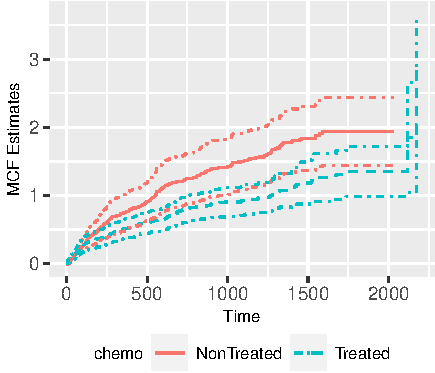
\includegraphics[scale = .60]{recur-figs/plot-sampleMcf-1}
        \caption{Stratified by \texttt{chemo}}
    \end{minipage}\hfill
    \begin{minipage}{0.24\textwidth}
        \centering
        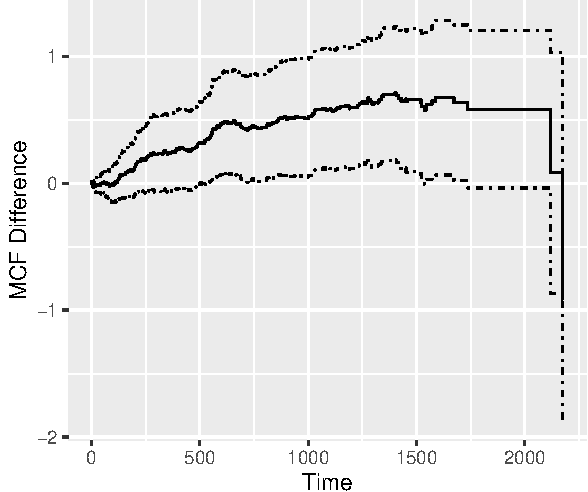
\includegraphics[scale = .45]{recur-figs/mcfdiffplot-1}
        \caption{MCF difference}
    \end{minipage}
\end{figure}

The MCF difference between two groups can be tested via
\texttt{mcfDiff.test()}, which implements the two-sample pseudo-score
tests of \citep{cook1996biometrics}. The following results indicate the
MCF estimates are statistically different at a significance level of
0.05. The MCF difference can be plotted with directly by
\texttt{plot(mcfDiff(re\_mcf))}, as shown in Fig. 4.

\begin{Shaded}
\begin{Highlighting}[]
\NormalTok{reda}\OperatorTok{::}\KeywordTok{mcfDiff.test}\NormalTok{(re\_mcf)}
\end{Highlighting}
\end{Shaded}

\begin{verbatim}
Two-Sample Pseudo-Score Tests:
                Statistic Variance  Chisq DF Pr(>Chisq)  
Constant Weight     47.49   416.71   5.41  1      0.020 *
Linear Weight       36.56   263.59   5.07  1      0.024 *
---
Signif. codes:  
0 '***' 0.001 '**' 0.01 '*' 0.05 '.' 0.1 ' ' 1

Variance Estimator: robust 
\end{verbatim}
